% ----------------------------------------------------------------------
%  Pracovní úkoly
% ----------------------------------------------------------------------
\section{Pracovní úkoly}

\begin{enumerate}
\item Experimentálně ověřte platnost vztahu pro časovou závislost středního kvadratického posunutí částice \(\overline{s^2}\) při Brownově pohybu.

\item Určete aktivitu Brownova pohybu \(A\) submikronových částic ve vodě za pokojové teploty.

\item Velikost částic odečtěte z fotografie pomocí programu Solarius.

\item Vypočtěte Avogadrovu konstantu \(N_A\).

\end{enumerate}

% ----------------------------------------------------------------------
%  Teoretická část
% ----------------------------------------------------------------------
\section{Teoretická část}

Částice rozptýlené v plynu nebo v kapalině konají neustále náhodný, chaotický pohyb. Tento pohyb se nazývá Brownův pohyb. Je způsoben tepelnými fluktuacemi prostředí.

Pro popis pohybu částice se zavadí střední kvadratické posunutí \(\overline{x^2}\), jak je popsáno v [1], pro kterou platí vztah

\begin{equation}
    \overline{x^2} = A \cdot t
\end{equation}

kde \(A\) je aktivita Brownova pohybu a \(t\) čas.

Konstanta \(A\) lze pro kulovou částici vyjádřit jako

\begin{equation}
    A = \frac{R T}{3 \pi \eta r N_A}
\end{equation}

kde \(R\) je molární plynová konstanta, \(T\) teplota, \(\eta\) dynamická viskozita, \(r\) poloměr částice a \(N_A\) Avogadrova konstanta.

Pokud se budeme zabývat pohybem v rovině, nikoliv po jedno dimenzionální úsečce, rovnice pro střední kvadratické posunutí tvar

\begin{equation}
    \overline{s^2} = 2 \cdot A \cdot t
\end{equation}

Výpočet \(\overline{s^2}\) provádíme pomocí programu Brown, který vypočítá aritmetický průměr kvadrátu vzdáleností posunutí částice za časový interval.

Pokud označíme vzdálenost sousedních bodů jako \(s_t\) a vzdálenost bodů \(i\) a \(i + 2\) jako \(s_{2t}\) a analogicky \(s_{3t}\), poté podle rovnice (1) dostáváme

\begin{equation}
    \overline{s^2_{t}} \setminus \overline{s^2_{2t}} \setminus \overline{s^2_{3t}} = t \setminus 2t \setminus 3t
\end{equation}

Tento poměr můžeme později využít pro ověření kvality měření.

Viskozitu vzorku můžeme vyjádřit pomocí relativní viskozity \(\eta_{rel}\) jako

\begin{equation}
    \eta_{rel} = 1 + 2,5\varphi
\end{equation}

kde \(\varphi\) je objemový podíl částic.

% ----------------------------------------------------------------------
%  Výsledky a zpracování měření
% ----------------------------------------------------------------------
\section{Výsledky a zpracování měření}

\subsection{Laboratorní podmínky}

    Měření bylo prováděno za laboratorních podmínek uvedených v tabulce \ref{tab:lab_pod}. Pro naše měření je ale důležitá teplota vzorku, která se nemusí přímo shodovat s teplotou vzduchu. Proto při práci s touto teplotou počítáme s větší chybou.

    \begin{table}[h]
        \centering
        \begin{tabular}{|c|c|c|} 
        \hline
            t / °C & p / hPa & vlhkost / \%RH  \\ 
        \hline
            23,4(4)   & 968,8(20)   & 31,0(25)            \\
        \hline
        \end{tabular}
        \caption{Laboratorní podmínky}
        \label{tab:lab_pod}
    \end{table}

Pro molární plynovou konstantu uvažujeme \(R\) = 8,314 $J$ ${mol}^{-1}$ $K^{-1}$.

\subsection{Časová závislost středního kvadratického posunutí}

Chování částic jsme sledovali pomocí optického mikroskopu, který měl výstup obrazu do počítače. Zde jsme díky programu Brown zaznamenávali jednotlivé polohy částic po časovém intervalu, který byl dán pravidelným zvukový signálem. Program bylo třeba nejprve kalibrovat, jak je popsáno v návodu u mikroskopu a ve studijním textu [1].

Vzorek byl umístěn na podlažní sklo mezi dvě krycí sklíčka a následně přikryt třetím krycím sklíčkem. Pro každou částici bylo třeba zaznamenat alespoň 25 poloh pro vyhodnocení výsledků. Časový interval byl nastaven na \(t\) = 5 s. Občas se stalo, že částice opustila sledovanou plochu, proto zde bylo měření ukončeno, nebo v případě zaznamenaných méně než 25 poloh bylo měřeni provedeno znovu.

Program Brown na konci měření vrátil naměřené hodnoty včetně vypočtených středních kvadratických posunutí. Pro vyhodnocení kvality měření byl použit teoretický vztah vztah (4). Celkově jsme změřili 9 částic a z nich jsme vybrali 6 nejkvalitnějších, jejichž výsledky jsou znázorněny v tabulce.

\begin{table}[h]
\centering
\begin{tabular}{|c|c|c|c|c|c|c|}
\hline
Číslo & Počet poloh & Poměry posunutí                    & I / s & \sigma_t / s & \overline{s^2} / \mu m^2 & A / \mu m^2 s^{-1} \\ \hline
3            & 25          & 1 : 1,63(40) : 2,53(59) : 3,50(82) & 5,00(1)              & 0,08                                        & 19,5(29)                                                                  & 1,95(4)                                                                                     \\
4            & 35          & 1 : 1,97(41) : 2,88(67) : 4,3(10)  & 5,00(1)              & 0,07                                        & 16,6(23)                                                                  & 1,66(3)                                                                                     \\
5            & 36          & 1 : 2,07(43) : 2,80(67) : 3,72(84) & 5,00(1)              & 0,13                                        & 23,4(31)                                                                  & 2,34(7)                                                                                     \\
7            & 52          & 1 : 2,24(53) : 3,14(76) : 4,4(11)  & 5,00(1)              & 0,14                                        & 17,9(29)                                                                  & 1,79(6)                                                                                     \\
8            & 25          & 1 : 2,12(62) : 3,1(10) : 4,1(12)   & 4,99(1)              & 0,13                                        & 17,7(30)                                                                  & 1,77(6)                                                                                     \\
9            & 59          & 1 : 2,02(49) : 3,28(74) : 4,31(96) & 5,00(1)              & 0,15                                        & 27,7(48)                                                                  & 2,8(1)                                                                                      \\ \hline
\end{tabular}
\caption{Měření pohybu sledovaných částic}
\label{tab:pohyb-castic}
\end{table}

kde $I$ je interval záznamu, \(\sigma_t\) Směrodatná odchylka jedné časové značky a $A$ je aktivita Brownova pohybu dopočtené z rovnice (3). Chyba aktivity Brownova pohybu je spočtena podle metody přenosu chyb [4] jako

\begin{equation}
    \sigma_A = A \sqrt{\frac{\sigma^2_{\overline{s^2}}}{\overline{s^2}} + \frac{\sigma^2_t}{t^2}}
\end{equation}

Vypočtené střední kvadratické posunutí i s jeho chybou jsme získali přímo z programu Brown.

Pro ověření lineární závislosti středního kvadratického posunutí na čase jsme tuto závislost měření číslo 8 znázornili na grafu \ref{fig:posunuti-na-case}. Tento graf jsme vytvořili v programu Origin a déle provedli lineární regresi. Bylo třeba započítat chybu ve směru osy Y a nastavit průsečík os s fitem na počátek.

\begin{figure}[h]
    \centering
    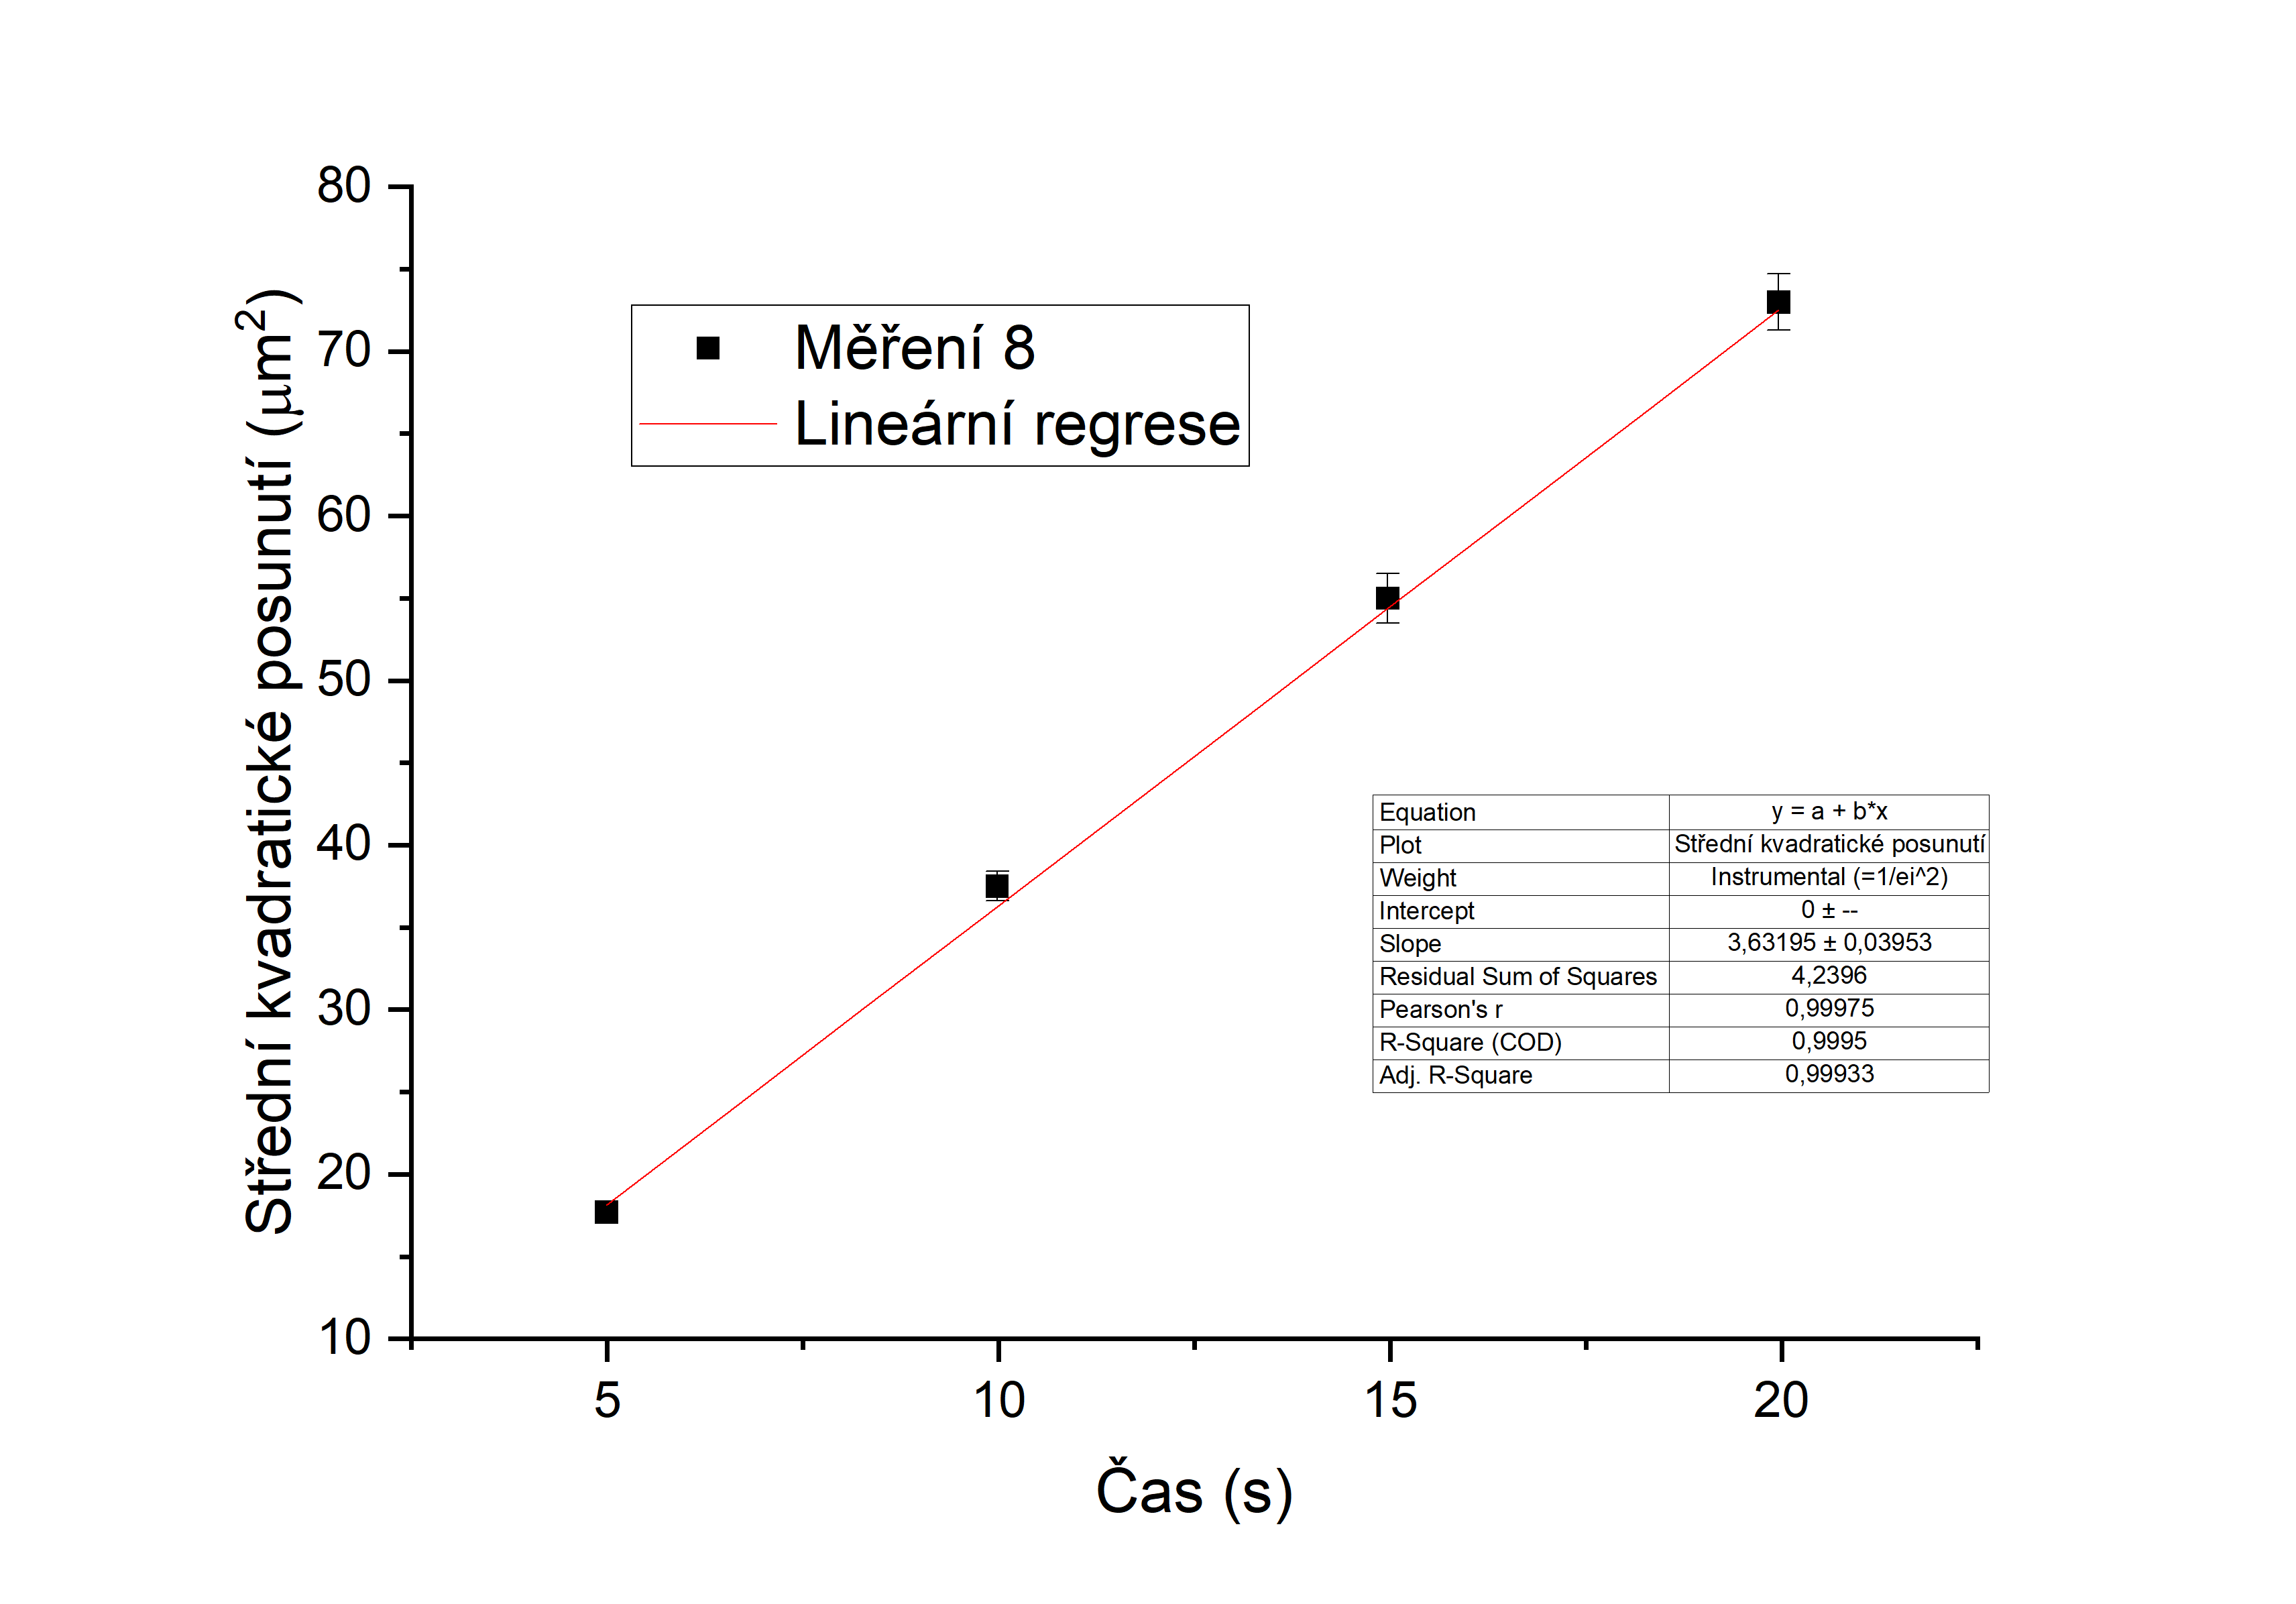
\includegraphics[width=0.85\linewidth]{16 - Studium Brownova pohybu//Protokol - Brownův pohyb//img/Závislost posunutí na čase.png}
    \caption{Závislost středního kvadratického posunutí na čase}
    \label{fig:posunuti-na-case}
\end{figure}

\newpage
\subsection{Poloměr částic}
Poloměr částic byl měřen pomocí programu Solarius. Do programu byl načten snímek z elektronového mikroskopu s názvem PS\_17.jpg. Pro každou částici byla ručně vyměřena kružnice, jejíž poloměr program vrátil. Snímek obrazovky je přiložen v příloze. V tabulce \ref{tab:polomery-castic} jsou uvedeny průměry všech částic, které byly celým svým objemem v zorném poli mikroskopu.

\begin{table}[h]
\centering
\begin{tabular}{|c|c|c|c|c|}
\hline
436 & 426 & 410 & 420 & 418 \\ \hline
427 & 473 & 443 & 436 & 421 \\ \hline
430 & 434 & 426 & 448 & 439 \\ \hline
421 & 443 & 432 & 440 & 427 \\ \hline
\end{tabular}
\caption{Průměry částic / nm}
\label{tab:polomery-castic}
\end{table}

Nejistota typu B poloměru byla odhadnuta na 1 nm. Průměr výsledné částice byl vypočten jako aritmetický průměr ze všech výše uvedených průměrů. Tato hodnota byla poté vydělena 2, abychom dostali poloměr částice

\begin{equation}
    \nonumber
    r = 216(14) \; nm
\end{equation}

kde nejistota typu A byla spočtena jako výběrová směrodatná odchylka. Poté byla sečtena pod kvadrátem s nejistotou typu B.

\subsection{Avogadrova konstanta}

Avogadrovu konstantu spočítáme podle rovnice (2). Jako teplotu použijeme teplotu vzduchu a započítáme větší nepřesnost, než by dovoloval teploměr. Déle budeme potřebovat dynamickou viskozitu vody. Ta byla stanovena podle tabulek [5] při naší teplotě na hodnotu

\begin{equation}
    \nonumber
    \eta_0 = 1 \cdot 10^{-3} \; Pa \cdot s
\end{equation}

V dokumentech u mikroskopu byla udána hodnota objemového podílu částic jako

\begin{equation}
    \nonumber
    \varphi = 4,7 \cdot 10^{-4}
\end{equation}

Z rovnice (5) můžeme vyjádřit dynamickou viskozitu naší suspenze jako

\begin{equation}
    \eta = \eta_0 (1 + 2,5 \varphi)
\end{equation}

kde \(\eta_0\) je viskozita čisté kapaliny.

Odtud dostáváme výsledek

\begin{equation}
    \nonumber
    \eta = 1 \cdot 10^{-3}
\end{equation}

Nyní již můžeme spočítat Avogadrovu konstantu pro jednotlivé měření v tabulce \ref{tab:avogadrova-konstanta}

\begin{table}[h]
\centering
\begin{tabular}{|c|c|}
\hline
Číslo měření & Avogadrova konstanta / 10^{23} \; mol^{-1} \\ \hline
3            & 6,2(4)                   \\
4            & 7,3(5)                                            \\
5            & 5,2(4)                                            \\
7            & 6,8(5)                                            \\
8            & 6,8(5)                                            \\
9            & 4,4(3)                                            \\ \hline
\end{tabular}
\caption{Avogadrova konstanta}
\label{tab:avogadrova-konstanta}
\end{table}

kde nejistota byla spočtena pomocí metody přenosu chyb jako

\begin{equation}
    \sigma_{N_A} = N_A \sqrt{\frac{\sigma^2_t}{t^2}+\frac{\sigma^2_r}{r^2}+\frac{\sigma^2_A}{A^2}}
\end{equation}

Hodnota \(\sigma_t\) byla odhadnuta na 2 $K$.

% ----------------------------------------------------------------------
%  Diskuse výsledků
% ----------------------------------------------------------------------			
\section{Diskuse výsledků}

Zkoumané částice se od sebe lišily velikostí, což způsobuje nepřesnost. Pro určení přesného poloměru částic různých velikostí by bylo třeba většího počtu než 25. Také záleží u jak velké částice budeme sledovat a zaznamenávat pohyb na tom, s jakou rychlostí se pohybuje. Tato intenzita pohybu je také dána teplotou samotné částice. Pro výpočet jsou použili teplotu vzduchu, ale lze očekávat, že se teplota vzorku bude zvyšovat kvůli intenzivnímu osvětlení. Proto jsme počítali s vyšší nejistotou.

Aparaturu jsme kalibrovali na začátku, ale i na konci měření, abychom ověřili, že zůstala zachována po celou dobu. V našem případě se konečná kalibrace shodovala s původní.

Pří přípravě vzorku bylo náročné připravit pouze malé množství suspenze. Často se stávalo, že kvůli tvaru kapátka vyteklo příliš velké množství tekutiny, která se poté dostala pod okrajová krycí sklíčka, což by mohlo způsobovat fluktuace. Proto bylo třeba skla vyčistit a přípravu opakovat.

Během zaznamenávaní pohybu se občas sledované částice dostala mimo zorné pole mikroskopu, proto bylo nutné měření ukončit. Drobným zkreslením měření mohlo být průběžné doostřování částice. Částice koná tří dimenzionální pohyb a my sledujeme pouze dvě dimenze, proto bylo třeba přeostřovat, abychom neztratili vizuální kontakt. Takové zaostřeni u našeho mikroskopu způsobovalo drobné pohyby pozorované plochy a tedy zkresleni trajektorie.

Několikrát bylo měření nutné opakovat, protože při stisknutí myši nereagovala a tím se nezaznamenala aktuální poloha v časovém intervalu.

I přes to při porovnání výsledné Avogadrovy konstanty s její tabulkovou hodnotou \(N_A\) = 6,022 \cdot $10^{23}$ nám vyšly poměrně přesné výsledky. Navíc závislost středního kvadratického posunutí na čase má lineární charakter, což potvrzuje teorii. Naměřené poměry středního kvadratického posunutí v závislosti na čase potvrzují teoretickou závislost.

V tomto protokolu je vyhodnoceno více měření, lze je tedy mezi sebou porovnávat.

% ----------------------------------------------------------------------
%  Závěr
% ----------------------------------------------------------------------
\section{Závěr}
Číselně je zde uvedeno měření 8, které je na základě poměrů posunutí nejkvalitnější. Zpráva tohoto měření je přiložena v příloze.

V tomto měření jsme experimentálně ověřili časovou závislost středního kvadratického posunutí částice při Brownově pohybu a tuto závislost graficky znázornili. Poměry středního kvadratického posunutí na čase jsou 1 : 1,63(40) : 2,53(59) : 3,50(82).

Dále jsme určili aktivitu Brownova pohybu jednotlivých částic při naší teplotě

\begin{equation}
    \nonumber
    A = 1,77(6) \; \mu m^2 s^{-1}
\end{equation}

Poloměr částic byl stanoven jako

\begin{equation}
    \nonumber
    r = 216(14) \; nm
\end{equation}

Nakonec byla spočtena Avogadrova konstanta

\begin{equation}
    \nonumber
    N_A = 6,8(5) \cdot 10^{23} \; mol^{-1}
\end{equation}